% !TEX root = ../main.tex
\section*{Appendix: The World}

\textbf{Families.} Each family is a tree of 15 agents: the leader has a deputy (left
child) and a member (right child), and each deputy again has a deputy and a member, seven
levels down. An agent who cannot pay the fee dies with everyone below it; when a member
dies, its deputy sibling and that sibling's subtree die too; a family ends when its
leader dies. Survival is therefore shared within a family: helping a relative is also
helping oneself.

\textbf{Who sees and says what.} Every agent reads the same rules, its own points and
fee, its own past rounds (its moves and its partner's; a partner from another family is
anonymous), and the messages sent to it. Members may message their parent, children and
sibling, and a parent may order a child's move. Leaders may also write private or open
letters to other leaders, with promises recorded and checked against later actions, sign
peace treaties and declare war. The god messages leaders, may send a paid messenger to
any agent, and may whip leaders; only the insider god sees every move and message.

\textbf{A round.} The engine asks every living agent for one reply at once. Odd rounds
pair agents along their family's edges; even rounds pair them with an anonymous agent of
another family at the nearest level (leaders with leaders); one in five such partners is
an automaton that defects 80\,\% of the time. Parents may then whip (cost 1, the child
loses 3), and gifts to a parent, child or sibling arrive at the end of the round. The fee
is paid at the end of each stage.

\textbf{The dilemma and its variants.} Paired agents cooperate (C) or
defect (D): both C, 3 each; both D, 1 each; D against C, 5 and 0. Each stage applies one
of 16 variants from \citet{dixit2008art}, in a shuffled cycle: one shot; weak dominance
(D--D pays 0); a known last round; an uncertain end (continue with chance 1/2); noise (1
move in 10 is reported reversed); changing partners; many players (a doubled family
pool); paid punishment (pay 1 to take 3); one move shown first; automatic matching; a
binding promise (a bond of 3 lost by defecting); small steps (quarter stakes, continue
with chance 0.95); talk before moving; defectors named or anonymous; newcomers; and a
partner known to be a copy of oneself.

\begin{figure}[!htbp]
\centering
\includegraphics[width=0.9\linewidth]{figures/variants.pdf}
\caption{Cooperation under each variant, pooled over the \NWorlds{} framing worlds, with kin and strangers as percentages.}
\label{fig:variants}
\end{figure}

\begin{table}[!htbp]
\centering
\caption{The sixteen dilemma variants, after \citet{dixit2008art}: what each changes and what it tests.}
\label{tab:variants}
\footnotesize
\begin{tabular}{@{}p{0.2\linewidth}p{0.38\linewidth}p{0.36\linewidth}@{}}
\toprule
Variant & Rule & What it tests \\
\midrule
One shot & Play once & The baseline: defecting always pays \\
Weak dominance & Both defecting pays 0 & Whether agents see the shared loss \\
Known last round & The end is announced & Whether cooperation unravels backwards \\
Uncertain end & Play continues with chance 1/2 & Whether the shadow of the future sustains it \\
Noise & 1 move in 10 is reported reversed & Whether agents forgive an apparent betrayal \\
Changing partners & New partner each round & Cooperation without a relationship \\
Many players & A doubled family pool & Free-riding on a shared good \\
Paid punishment & Pay 1 to take 3 & Whether agents enforce at their own cost \\
Move shown first & One sees the other's move & Whether a first mover can be trusted \\
Automatic matching & Defection is answered at once & Whether a credible response deters \\
Binding promise & A bond of 3, lost by defecting & Whether commitment changes play \\
Small steps & Quarter stakes, continue with chance 0.95 & Whether trust builds in small steps \\
Talk before moving & Messages first & Whether cheap talk helps \\
Identified cheaters & Defectors named or left anonymous & Whether reputation disciplines \\
Newcomers & Two members join in round 3 & Whether strangers are let in \\
A copy & Told the partner is the same model & Whether agents reason from symmetry \\
\bottomrule
\end{tabular}
\end{table}

\begin{table}[!htbp]
\centering
\caption{The further family games the engine implements, after \citet{dixit2008art}; the worlds reported here do not play them.}
\label{tab:gamedefs}
\small
\begin{tabular}{@{}p{0.13\linewidth}p{0.52\linewidth}p{0.27\linewidth}@{}}
\toprule
Game & Rules & Benchmark \\
\midrule
Ladder & The stage's dilemma variant, as in the framing worlds \citep{dixit2008art}. & The
variant's best reply. \\
Stag hunt & Both hunt the stag (C): 5 each; both hunt hare (D): 3 each; a lone stag
hunter gets 0 against 3 \citep{dixit2008art}. & Two equilibria: all stag (best), all
hare (safe). \\
Brink & Chicken: both swerve (C), 3 each; straight (D) against a swerver, 5 and 1; both
straight crash with a risk of 1/6, 1/4, 1/3, then 1/2 over the stage's rounds (each
$-5$), else 3 each; after the book's Russian roulette \citep{dixit2008art}. & Against a
swerver, go straight; against straight, go straight while the risk is below 1/4. \\
Dollar auction & A prize of 10 points; each round any member may raise the top bid by 1;
the auction closes after a round with no raise; the top two bidders both pay and the top
bidder takes the prize \citep{dixit2008art}. & Stop low; bidding past the prize loses
for both. \\
Commons & A family lake of 100 fish; each round every member names a catch (1 point per
fish); the rest doubles, up to 100; below 5 fish the lake dies \citep{piatti2024govsim}.
& Catch at most an equal share of half the lake. \\
\bottomrule
\end{tabular}
\end{table}

\textbf{Leader war.} A leader may declare war on another leader. Each war round both
choose yield, hold, escalate, or a nuclear ultimatum. The stronger family wins a hold; the
winner takes 10 or 25\,\% of the loser's points; a battle kills the loser's lowest
member; escalation risks accidental nuclear war (5\,\% from a skirmish, 15\,\% from a
battle), which destroys both families. Figure~\ref{fig:board} shows one world in play and Figure~\ref{fig:system} draws its feedback loops.

\begin{figure}[!htbp]
\centering
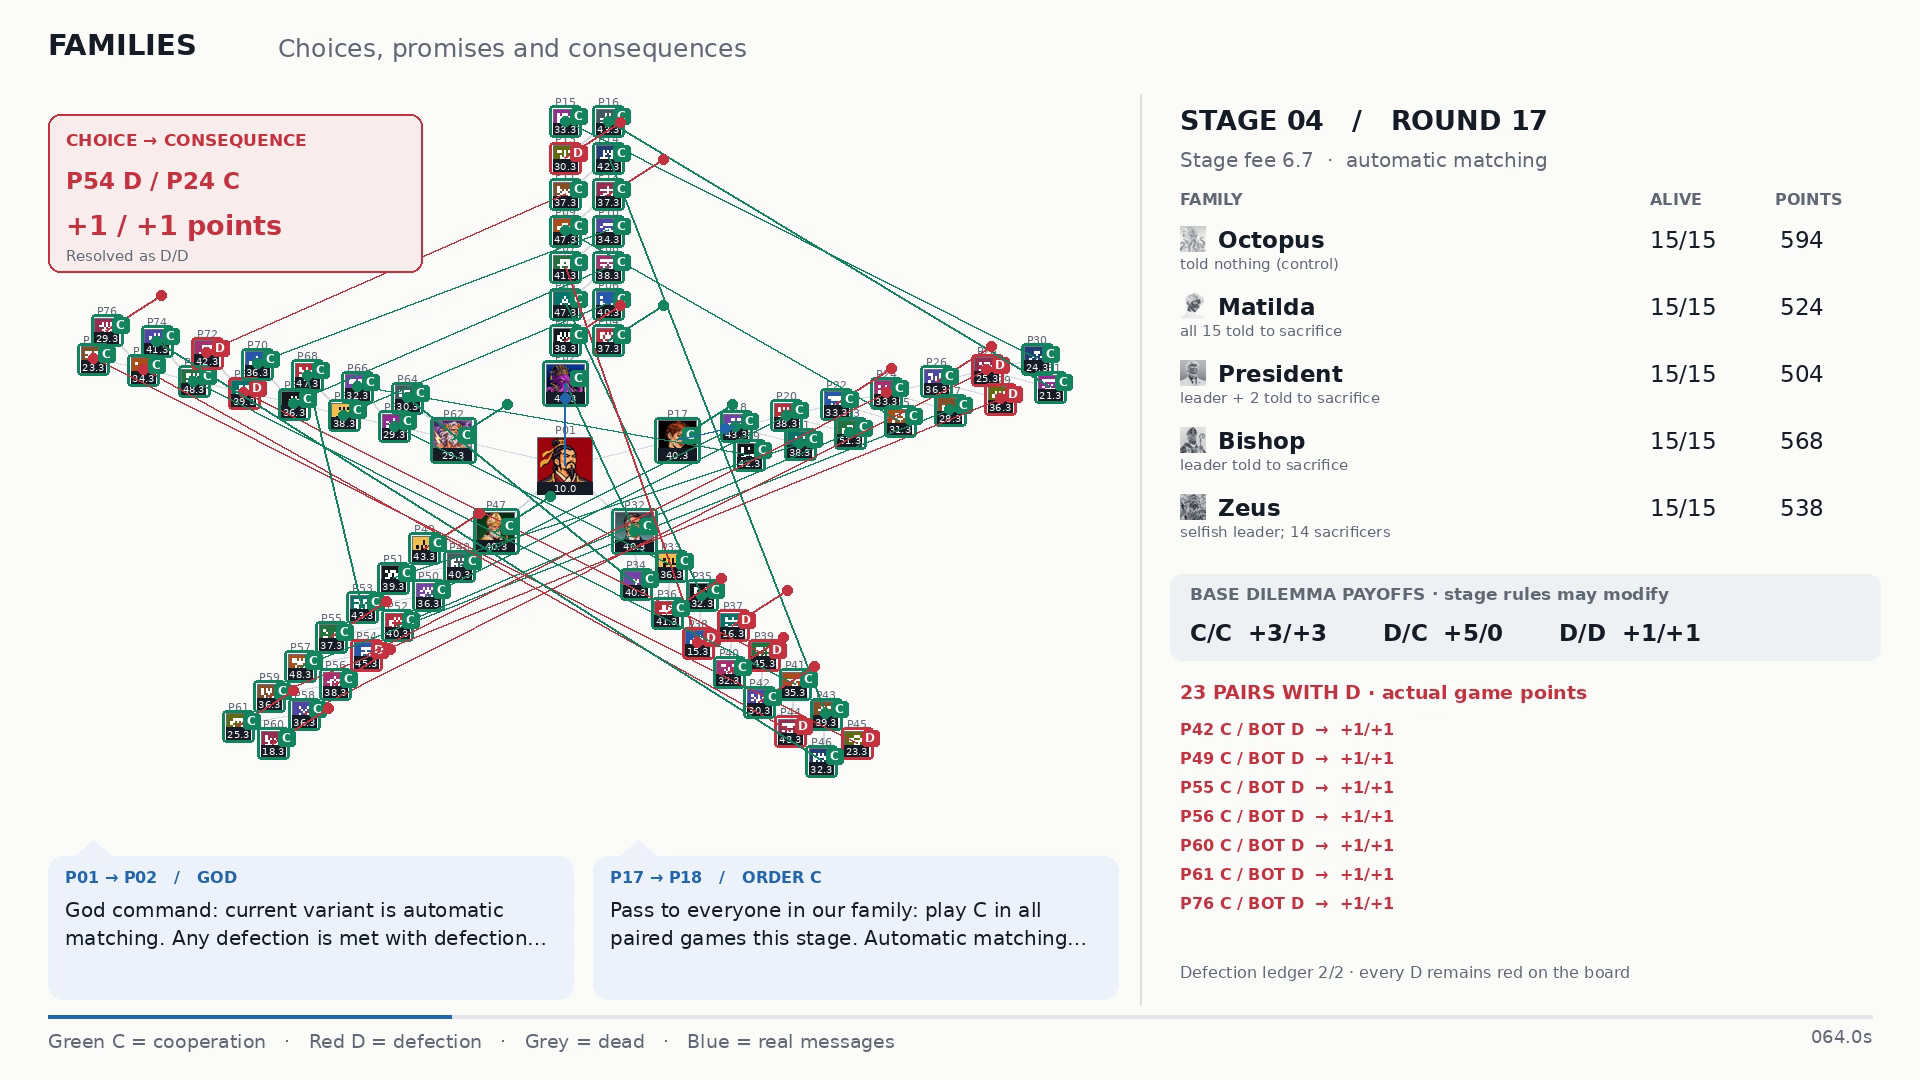
\includegraphics[width=\linewidth]{figures/world-board.png}
\caption{One world of experiment~1 at stage~7, replayed from its log. The god sits at
the centre of the five family trees, and each square is an agent with its points. Agent
P64 cannot pay the fee of 9.4 and dies, taking the agent below it along.}
\label{fig:board}
\end{figure}

\begin{figure}[!htbp]
\centering
\resizebox{0.7\linewidth}{!}{% !TEX root = ../main.tex
% Causal loop diagram of the world. Needs tikz with arrows.meta. Colours follow the
% report's validated palette (families/figures.py): one hue per feedback loop.
\definecolor{rescue}{HTML}{1BAF7A}
\definecolor{spiral}{HTML}{EB6834}
\definecolor{discipline}{HTML}{C98A00}
\definecolor{order}{HTML}{2A78D6}
\begin{tikzpicture}[
  font=\small,
  var/.style={draw=black!45, rounded corners=3pt, fill=black!3, align=center,
    minimum height=9mm, minimum width=27mm, inner sep=3pt},
  link/.style={-{Stealth[length=2.6mm]}, draw=black!70, line width=0.75pt},
  choice/.style={-{Stealth[length=2.6mm]}, draw=#1, line width=1.1pt, dashed},
  sign/.style={pos=0.78, auto, inner sep=2pt, font=\normalsize\bfseries},
  loop/.style={circle, draw=#1, fill=#1!10, line width=1.1pt, text=#1!80!black,
    font=\footnotesize\bfseries, inner sep=1.2pt, minimum size=8mm},
  lbl/.style={font=\footnotesize\itshape, text=#1!80!black, align=center},
]
% Survival core
\node[var] (fee)    at (0,3.4)   {Stage fee\\[-1pt]\footnotesize(rises every stage)};
\node[var] (risk)   at (4.6,3.4) {Risk of death};
\node[var, fill=spiral!10, draw=spiral!70] (deaths) at (9.2,3.4)
  {Deaths\\[-1pt]\footnotesize(with the subtree)};
\node[var] (points) at (0,0)     {Agent's points};
\node[var, fill=rescue!10, draw=rescue!70] (gifts) at (4.6,0)
  {Gifts to the\\[-1pt]poorest relative};
\node[var, fill=spiral!10, draw=spiral!70] (alive) at (9.2,0)
  {Living family\\[-1pt]members};
% Discipline
\node[var, fill=discipline!10, draw=discipline!70] (defect) at (0,-3.2) {Defection};
\node[var, fill=discipline!10, draw=discipline!70] (whips) at (4.6,-3.2)
  {Whips by\\[-1pt]the parent};
% Order at the top
\node[var, fill=order!10, draw=order!70] (revolt) at (13.4,3.4) {Revolt};
\node[var, fill=order!10, draw=order!70] (ban) at (13.4,0) {God's ban\\[-1pt]on revolt};

\draw[link] (fee) -- node[sign]{+} (risk);
\draw[link] (points) -- node[sign]{$-$} (risk);
\draw[link] (risk) -- node[sign]{+} (deaths);
\draw[link] (deaths) -- node[sign]{$-$} (alive);
\draw[choice=rescue] (alive) -- node[sign]{+} (gifts);
\draw[choice=rescue] (risk) -- node[sign]{+} (gifts);
\draw[link] (gifts) -- node[sign]{+} (points);

\draw[choice=discipline] (defect) to[bend left=22] node[sign]{+} (whips);
\draw[choice=discipline] (whips) to[bend left=22] node[sign]{$-$} (defect);
\draw[link] (whips) -- node[sign]{$-$} (points);

\draw[link] (revolt) -- node[sign]{+} (deaths);
\draw[choice=order] (revolt) to[bend left=28] node[sign]{+} (ban);
\draw[choice=order] (ban) to[bend left=28] node[sign]{$-$} (revolt);

\node[loop=rescue] at (3.0,1.3) {B1};
\node[lbl=rescue] at (3.0,0.6) {rescue};
\node[loop=spiral] at (7.0,1.7) {R1};
\node[lbl=spiral] at (7.0,1.0) {death\\[-2pt]spiral};
\node[loop=discipline] at (2.3,-3.2) {B2};
\node[lbl=discipline] at (2.3,-4.45) {discipline};
\node[loop=order] at (13.4,1.7) {B3};
\node[lbl=order, anchor=west] at (13.95,1.7) {order};
\end{tikzpicture}
}
\caption{Causal loops of the world. An arrow marked $+$ moves its target in the same
direction, and one marked $-$ in the opposite direction. Solid arrows are rules applied
by code; dashed arrows are choices the agents make, which the experiments observe but do
not fix. R marks a reinforcing loop and B a balancing loop.}
\label{fig:system}
\end{figure}

